\documentclass{article}
\usepackage[utf8]{inputenc}
\usepackage{graphicx}
\usepackage{siunitx}
\usepackage{caption}

\newcommand{\source}[1]{\hfill \footnotesize \caption*{Source: {#1}} }

\title{
\includegraphics[width=0.5\textwidth]{UU_logo.pdf}\\
Construction of the Slidarr}

\author{Mats Jonsson, Sören Meinken, Mohammad El Musleh}
\date{May 2019}

\begin{document}

\maketitle

\pagebreak

\tableofcontents

\pagebreak

\section{Background}
Blabla blabla bla.

\section{Analysis}

\subsection{Resistance measurement}
One way of determining the finger's position of the string is to measure the resistance from one end of the string to the finger. A copper wire of length 1 meter and diameter of \SI{0.5}{mm} has a resistance of \SI{0.5}{\ohm} per meter \cite{copperresistance}. In order to track the position  with millimeter accuracy, we need to measure in the sub-\si{\milli\ohm} range. 

This can be done in many different ways. One way is using a resistor bridge setup, e.g. a Wheatstone or Kelvin bridge, which is able to sense tiny changes in resistance. However, the bridge needs to be balanced with accurate resistors of similar value of the measured resistor, which is hard to achieve with standard resistors when the measured resistance is this small.

\begin{figure}[ht]
  \centering
  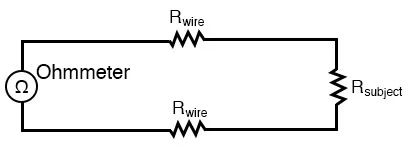
\includegraphics[width=0.5\textwidth]{4-wire-sensing}
  \caption{4-terminal measurement}
  \source{allaboutcircuits.com}
  \label{fig:4terminal}
\end{figure}

An more suitable method is to use four-terminal measurement as shown in figure \ref{fig:4terminal}. A known constant currenti $I$ is fed through the resistor with unknown resistance $R$, and the voltage drop $V$ is measured with a separate pair of wires. The resistance can then easily be calculated using Ohms law, $ R = V / I $.

\subsection{Voltage measurement}
Using four-terminal measurement with a current of \SI{100}{\milli\ampere}, the change in voltage per millimeter string is \SI{50}{\micro\volt}. This has now turned into a matter of measuring low-level voltages.

A 12-bit ADC operating at \SIrange{0}{3.3}{\volt} has a resolution of \SI{0.8}{\milli\volt} per bit. The signal needs to be amplified by at least 16 times in order to achieve \si{\milli\meter} accuracy.

\subsubsection{Instrumentation amplifier}
Since we are interested in the voltage difference over the string, a differential amplifier is a good choice for amplifying the signal. The \textit{instrumentation amplifier} is widely used for amplifying low-level signals. It is stable and easy to adjust, since the amplification can be set by a single resistor \cite{in}.

\subsection{The MIDI protocol}
MIDI (Musical Instrument Digital Interface) protocol is the industry standard for communication between electronic musical instruments and synthesizers \cite{midiorg}. It does not transport the audio itself, instead messages with instructions about the note, its volume and duration are sent to a receiving device which generates the sound. 

MIDI was designed to be used with digital piano keyboards. The messages indicate \textit{note on}, \textit{note off}, and their \textit{velocity} (volume). The protocol is built around the concept of piano notes, which is not optimal for the Slidarr since it operates at a continous scale rather than at fixed frequency intervals.

The solution to this is the \textit{pitchbend} message, which is usually controlled by a wheel controller on the keyboard. It is a global parameter that bends the pitch (offsets the frequency) of the currently played notes, on synths that support it. The amount of bending is not standardized and can differ between synthesizers.

The MIDI message consists of three bytes: the \textit{command} and two \textit{parameters} \cite{midistanford}. There are many different commands, but the Slidarr only needs the three as shown in table \ref{table:midi_msgs}.

\begin{table}[h]
  \centering
  \caption{MIDI messages}
  \label{table:midi_msgs}
  \begin{tabular}{llll}
    Action     & Command & Parameter 1 & Parameter 2 \\ \hline
    Note off   & 0x80    & Key         & Velocity    \\
    Note on    & 0x90    & Key         & Velocity    \\
    Pitch bend & 0xE0    & Value       & Value      
  \end{tabular}
\end{table}

\subsection{Sound generation}
A synthesizer has to be used to generate the sound from the MIDI messages. 

\section{Design}

\subsection{Interface}

\subsection{Electronics}

\section{Implementation}

\subsection{Making MIDI continuous}

\subsection{The state machine}

\subsection{Streaming MIDI}

\subsection{Wireless bridge}

\section{Testing and verification}

\section{Results}



\begin{thebibliography}{9}

\bibitem{copperresistance} 
Chemandy Electronics: Round Wire Resistance Calculator,
\\\texttt{https://chemandy.com/calculators/round-wire-resistance-calculator.htm}

\bibitem{in} 
Electronics Hub: Instrumentation Amplifier Basics and Applications,
\\\texttt{https://www.electronicshub.org/instrumentation-amplifier-basics-applications}

\bibitem{midiorg} 
The MIDI Association,
\\\texttt{https://www.midi.org}

\bibitem{midistanford}
Stanford CCRMA: Essentials of the MIDI protocol,
\\\texttt{https://ccrma.stanford.edu/~craig/articles/linuxmidi/misc/essenmidi.html}

\end{thebibliography}
\end{document}
